\chapter{操作系统OS}
\section{进程和线程的区别}
进程:进程是程序实体的运行过程,是系统进行资源分配和调度的一个独立单位;引入进程是为了使多个程序可以并发的执行,以提高系统资源的利用率和吞吐量。\\
线程:是比进程更小的可独立运行的基本单位,可以看做是轻量级的进程;引入的目的是为了减少程序在并发执行过程中的开销,使OS的并发效率更高。\\
\section{进程状态}
进程的状态有分为3、5、7种状态,其中三状态如下:
\begin{itemize}
\item 就绪状态:进程获得除CPU以外的所有必要资源,只要获得CPU就可以立即执行。
\item 执行状态:进程已经获得CPU,正在运行的状态。
\item 阻塞状态:处于执行状态的进程由于发生某些事件而暂时无法继续执行,放弃处理机而处于暂停状态。
\end{itemize}
\begin{figure} 
\centering
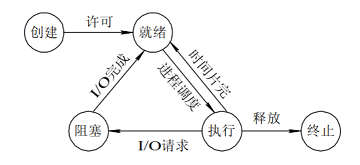
\includegraphics[width=12cm,height=10cm]{Image/chp3_2.png}
\caption{This is a pthread state}
\label{fig:pthread}
\end{figure}
\section{进程间通信}
\begin{itemize}
\item 管道:管道是一种半双工的通信方式,数据只能单向流动,而且只能在具有亲缘关系的进程间使用,即父子进程间。
\item 有名管道:同样是管道的一种,但是可以允许无亲缘关系进程间通信。
\item 信号量:信号量是一个计数器,可以用来控制多个进程对共享资源的访问。它常作为一种锁机制,防止某进程正在访问共享资源时,其他进程访问该资源。因此,主要作用是进程以及同一进程下的线程之间同步手段。
\item 消息队列:消息队列是消息的链表,存放在内核中并由消息队列标识符标识。消息队列克服了信号传递信息少、管道只能承载无格式字符流以及缓冲区大小限制等缺点。
\item 信号:信号是一种比较复杂的通信方式,用于通知接收进程某个事件以发生。
\item 共享内存:共享内存就是映射一段能被其他进程所访问的内存,这段共享内存由一个进程创建,但多个进程都可以访问。共享内存是最快的IPC方式,它是针对其他进程间通信方式运行效率低而专门设计的。
\item 套接字:套接字同样是进程通信机制一种,可以用于不同进程通信。
\end{itemize}
\section{孤儿进程和僵尸进程}
孤儿进程:一个父进程退出,而它的一个或多个子进程还在运行,那么这些子进程将成为孤儿进程。孤儿进程将被init进程所收养,并由init进程对其完成状态收集工作。\\
僵尸进程:一个进程使用fork创建子进程,如果子进程退出,而父进程并没有调用wait或waitpid获取子进程的状态信息,那么子进程的进程描述符仍然保存在系统中。这种进程称之为僵尸进程。
\section{系统函数}
\begin{itemize}
\item fcntl:文件控制
\item open:打开文件
\item create:创建文件
\item close:关闭文件套接字
\item read:读文件
\item write:写文件
\item readv:从文件读入数据到缓冲组中
\item writev:将缓冲组里的数据写入文件
\item pread:对文件随机读
\item pwrite:对文件随机写
\end{itemize}
\section{子进程与父进程不同点}
使用fork函数得到的子进程从父进程里继承了整个进程的地址空间,包括:进程上下文、进程堆栈、内存信息、打开文件描述符、信息控制设置、进程优先级、进程组号、当前工作目录、根目录、资源限制、控制终端等。\\
子进程和父进程的不同有:
\begin{itemize}
\item 父进程设置的锁,子进程不继承。
\item 各自进程ID和父进程ID不同。
\item 子进程的未决告警被清除。
\item 子进程的末决信号集设置为空集。 
\end{itemize}
\section{进程内存结构}
进程在内存的结构如下分配:
\begin{itemize}
\item 代码段:代码段是用来存放可执行文件的操作指令,也就是说它是可执行程序在内存中的镜像。代码段需要防止运行时被非法修改,所以只准许读操作,而不允许写入操作。
\item 数据段:数据段用来存放可执行文件中的已初始化全局变量,即存放静态分配的变量和全局变量。
\item BSS段:BSS段包含了程序中未初始化全局变量,在内存中BSS段全部置零。
\item 堆:堆是存放进程运行中被动分配的内存段,它的大小不固定,可动态扩张或收缩。
\item 栈:栈是用户存放临时创建的全局变量,也就是我们函数中定义的局部变量。
\end{itemize}

